
% \begin{thm}
% 	\label{thm:good_covers_theorem}
% 	If $ \U$, $\U'$ are \textbf{good covers} of $ X$ with associated Cech complexes $ \L^\bullet(\U)$ and $ \L^\bullet(\U')$ then
% 	\begin{align}
% 		H^i(\L(\U)) \cong  H^i(\L(\U'))
% 	\end{align}
% 	for all $ i \in \Z$ i.e. the cohomology of the Cech complex is independent of the good cover and hence is an invariant of the underlying space. Hence, we can define the Cech cohomology of $ X$ as
% 	\begin{align}
% 		\check H^i(X; \F) :=  H^i(\L(\U))
% 	\end{align}
% 	for any good cover $ \U$ of $ X$.
% \end{thm}


\subsection{Locally Constant Functions}
\begin{definition}
  For a topological space $ X$, let $ \L(X)$ denote the space of set maps $ f: X \rightarrow \F$ which are constant on each connected component of $ X$. Such functions are called \textbf{locally constant functions}.\footnote{$\L$ is an example of a \textbf{locally constant sheaf}, more on this later. }
\end{definition}
\begin{ques}
  Prove that if  $ X$ has $ k$ connected components $ X_1, \dots, X_k$ then as an $ \F$ vector space
  \begin{align*}
    \L(X) \cong \F^k
  \end{align*}
  Further, $ \L(X)$ has a \textbf{canonical basis} given by functions $ f_1, \dots, f_k$ defined as
  \begin{align*}
    f_i(X_j) & \equiv
    \begin{cases}
      1 & \mbox{ if } i=j \\ 0 & \mbox{ otherwise }
    \end{cases}
  \end{align*}
\end{ques}

\begin{ques}
  What is $ \L(X)$ if $ X$ is the empty set?
\end{ques}

\begin{ques}
  Show that if we think of $ \F$ as a disjoint union of two points then $ \L(X)$ is precisely the space of continuous functions $ X \rightarrow \F$. (We'll see later that this is the reason why $\L$ is a sheaf.)
\end{ques}


% \begin{definition}
%   For a topological space $ X$, let $ \L(X)$ denote the space of functions $ f: X \rightarrow \F$ which are constant on each connected component of $ X$. Such functions are called \textbf{locally constant functions}.
% \end{definition}
%
% \begin{ques}
%   Show that if we think of $ \F$ as a disjoint union of two points then $ \L(X)$ is precisely the space of continuous functions $ X \rightarrow \F$.
% \end{ques}
%
% \begin{ques}
%   Prove that if  $ X$ has $ k$ connected components $ X_1, \dots, X_k$ then as an $ \F$ vector space
%   \begin{align}
%     \L(X) \cong \F^k
%   \end{align}
%   Further, $ \L(X)$ has a \textbf{canonical basis} given by functions $ f_1, \dots, f_k$ defined as
%   \begin{align}
%     f_i(X_j) &\equiv
%     \begin{cases}
%       1 & \mbox{ if } i=j \\ 0 & \mbox{ otherwise }
%     \end{cases}
%   \end{align}
% \end{ques}
%
% \begin{ques}
%   What is $ \L(X)$ if $ X$ is the empty set?
% \end{ques}


\begin{ques}
  \label{q:gluing_diagram}
  We can construct a 2 holed torus $M^2$ by gluing the sides of an octagon as in Figure \ref{fig:genus2}. Use the gluing diagram to construct a good cover of $M^2$. Find the cohomology using this good cover.
\end{ques}

\begin{figure}[h]
	\centering
	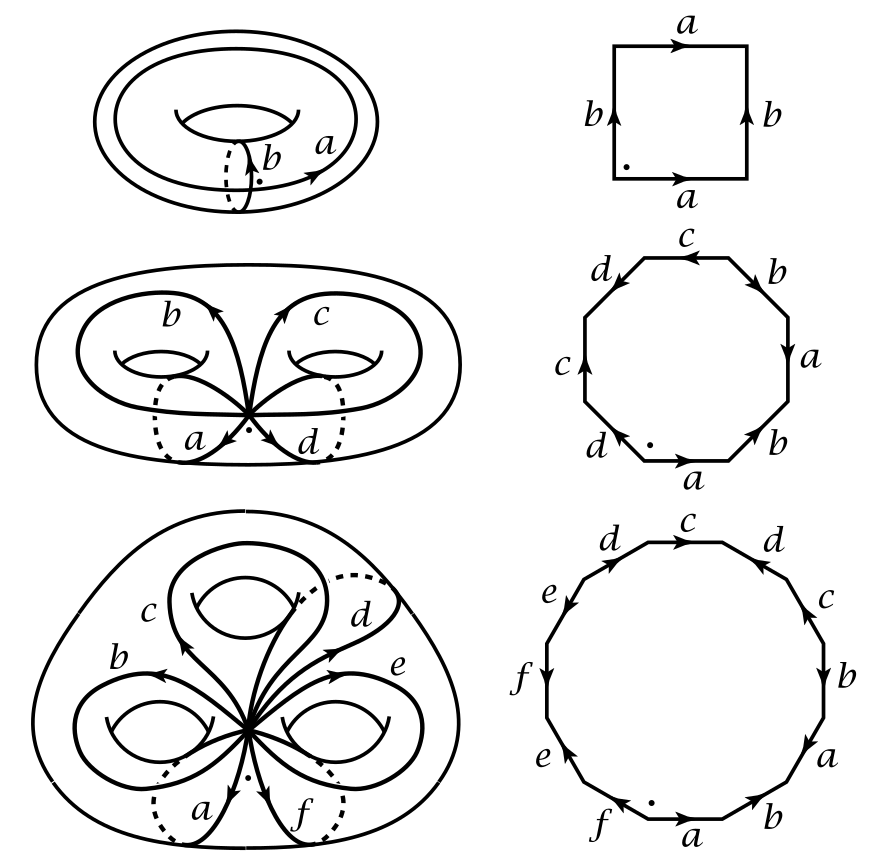
\includegraphics[width=11cm]{GluingDiagramHatcher}
	\caption{Constructing a $g$ holed torus $M^g$ using a $4g$-gon. (Image from Hatcher.)}
  \label{fig:genus2}
\end{figure}
\begin{ques}*
  More generally, it is possible to construct a $g$ holed torus by gluing polygons of $4g$ sides. Repeat Question \ref{q:gluing_diagram} for this surface.
\end{ques}


\begin{figure}[H]
	\centering
	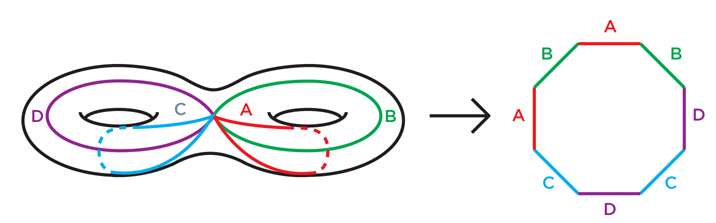
\includegraphics[width=11cm]{Genus2}
	\caption{Gluing diagram for constructing a 2 holed torus $M^2$ using an octagon. (Googled image.)}
  \label{fig:genus2}
\end{figure}

\begin{ques}
  By gluing the sides of a square in funky ways we can create the Klein Bottle and the Real Projective Plane. Find their Cech Cohomologies.
  \begin{figure}[H]
  	\centering
  	\begin{subfigure}[t]{0.4\textwidth}
  		\centering
  		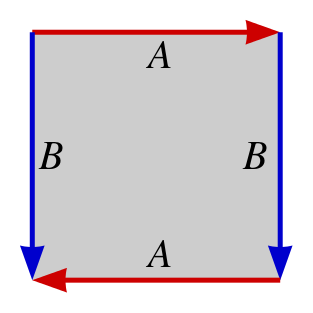
\includegraphics[height=3cm]{KleinBottle}
      \caption{Klein Bottle}
  	\end{subfigure}
  	\begin{subfigure}[t]{0.59\textwidth}
  		\centering
  		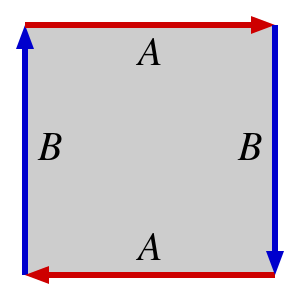
\includegraphics[height=3cm]{ProjectivePlane}
      \caption{Projective Plane}
  	\end{subfigure}
  \end{figure}
\end{ques}
